\section*{Exercice 1}
\setcounter{subparagraph}{0}
On démontre que sur l'ensemble $\mathbb{N}\times \mathbb{N}$ est dénombrable en numérotant chaque couple $(x,y)\in\mathbb{N}^2$ suivant le procédé suggéré par la figure ci-dessous.
\ifprof
\begin{center}
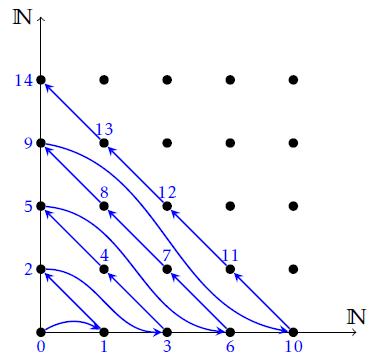
\includegraphics[width=.2\linewidth]{images/fig_01}
\end{center}
\else
\begin{center}
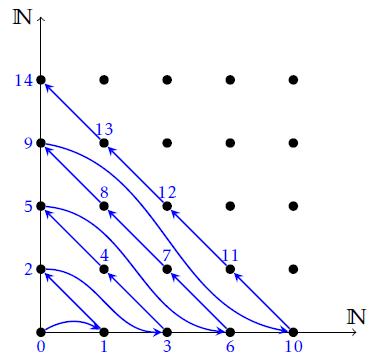
\includegraphics[width=.45\linewidth]{images/fig_01}
\end{center}
\fi

\subparagraph{}\textit{Rédiger une fonction récursive qui retourne le numéro du point de coordonnées $(x,y)$.}
\ifprof
\begin{corrige}
\begin{python}
def numerote(x, y):
    if x == 0 and y == 0:
        return 0
    if y > 0:
        return 1 + numerote(x+1, y-1)
    return 1 + numerote(0, x-1)
\end{python}
\end{corrige}
\else
\fi

\subparagraph{}\textit{Rédiger la fonction réciproque, là encore de façon récursive.}
\ifprof
\begin{corrige}
\begin{python}
def reciproque(n):
    if n == 0:
        return (0, 0)
    (x, y) = reciproque(n-1)
    if x > 0:
        return (x-1, y+1)
    return (y+1, 0)
\end{python}
\end{corrige}
\else
\fi



\section*{Exercice 2}
\setcounter{subparagraph}{0}
\subparagraph{}
\textit{Écrire une fonction récursive qui calcule $a^n$ en exploitant la relation : $a^n=a^{n/2}\times a^{n/2}$.}
\ifprof
\begin{corrige}
\begin{python}
def power(a, n):
    if n == 0:
        return 1
    elif n == 1:
        return a
    return power(a, n//2) * power(a, n-n//2)
\end{python}
\end{corrige}
\else
\fi

\subparagraph{}
\textit{Écrire une fonction qui utilise de plus la remarque suivante :}
$n/2 = \left\{ 
\begin{array}{ll} 
n/2 & \text{si }n \text{ est pair} \\
n/2+1 & \text{sinon}\\
\end{array}
\right.
$.
\ifprof
\begin{corrige}
\begin{python}
def power(a, n):
    if n == 0:
        return 1
    elif n == 1:
        return a
    x = power(a, n//2)
    if n % 2 == 0:
        return x * x
    else:
        return x * x * a
\end{python}
\end{corrige}
\else
\fi


\subparagraph{}
\textit{Déterminer le nombre de multiplications effectuées dans le cas où $n$ est une puissance de 2, et majorer 
simplement ce nombre dans le cas général.}
\ifprof
\begin{corrige}
On note $C(n)$ le nombre multiplications.

Dans le premier cas, on note $n=2^k$ et on conjecture que $\forall n>2, C(n)=k-1=\ln_2 (n)-1$ et on raisonne par 
récurrence.

Dans le second cas, on conjecture que $\forall n>2, C(n)\leq 2\ln_2 n$ et on raisonne par récurrence. En effet, le 
variant est $\ln_2 n$, qui diminue d'au moins 1 à chaque appel récursif. Il y a donc au plus $\ln_2 n$ appels 
récursifs. Or, il y a au plus 2 multiplications par appel.
\end{corrige}
\else
\fi



\section*{Exercice 3 -- Fonction 91 de McCarthy}
On considère la fonction récursive suivante : 
\begin{py}
\begin{python}
def f(n) :
    if n>100 : 
        return n-10
    return f(f(n+11))
\end{python}
\end{py}

\subparagraph*{} \textit{Prouver sa terminaison lorsque $n\in\mathbb{N}$ et déterminer ce qu'elle calcule (sans utiliser l'interpréteur de commande).}
\ifprof
\begin{corrige}

Distinguons plusieurs cas.

\begin{itemize}
\item Si $n\geq 101$, l'algorithme se termine et renvoie $n-10$. 
\item Si $n\in\llbr90, 100\rrbr$, montrons par récurrence descendante que le calcul de $f(n)$ termine et renvoie 
91.\\
C'est immédiat pour $n=100$ : $f(100)=f(f(111))=f(101)=91$.\\
Soit $n\in\llbr91,100\rrbr$ tel que $f(n)=91$. Alors $f(n-1)=f(f(n+10))=f(n)$ car $n+10>100$ donc $f(n+10)=n$. La 
propriété est 
donc héréditaire.\\
On raisonne ensuite par récurrence descendante de 10 en 10 : si $n\in\llbr80,89\rrbr$, alors $n+11\in\llbr90,100\rrbr$, 
donc $f(n)=f(f(n+11))=f(91)=91$ d'après le cas précédent. Et ainsi de suite pour les intervalles 
$\llbr70,79\rrbr\cdots\llbr0,9\rrbr$.
\end{itemize}
\end{corrige}


\else
\fi
%\section*{Exercice 2}
%\subparagraph*{}\textit{Prouver la terminaison de la fonction $G$ de Hofstadter, définie sur $\mathbb{N}$ de la façon suivante :}
%\begin{py}
%\begin{python}
%def g(n) :
%    if n== 0 : 
%        return 0
%    return n-g(g(n-1))
%\end{python}
%\end{py}

%
%\section*{Exercice 4}
%\setcounter{subparagraph}{0}
%On suppose donné un tableau $t[0,.., n-1]$ (contenant au moins trois éléments) qui possède la propriété suivante : $t_0\geq t_1$ et $t_{n-2}\leq t_{n-1}$. Soit $k\in[|1,n-2|]$; on dit que $t_k$ est un minimum local lorsque $t_k\leq t_{k-1}$ et $t_k\leq t_{k+1}$.
%
%\subparagraph{}\textit{Justifier l'existence d'un minimum local dans $t$.}
%\subparagraph{}\textit{Il est facile de déterminer un minimum local en coût linéaire : il suffit de procéder à un parcours de tableau. Pourriez-vous trouver un algorithme récursif qui en trouve un en réduisant le coût logarithmique?}

%\section*{Exercice 4}
%\setcounter{subparagraph}{0}
%
%Les processeurs graphiques possèdent en général une fonction de bas niveau appelée \textit{blit} (ou transfert de bloc) qui copie rapidement un bloc rectangulaire d’une image d’un endroit à un autre.
%
%L’objectif de cet exercice est de faire tourner une image carrée de $n\times n$ pixels de 90\textdegree dans le sens direct en
%adoptant une stratégie récursive : découper l’image en quatre blocs de tailles $n/2 \times n/2$, déplacer chacun des ces
%blocs à sa position finale à l’aide de 5 \textit{blits}, puis faire tourner récursivement chacun de ces blocs.
%
%\begin{center}
%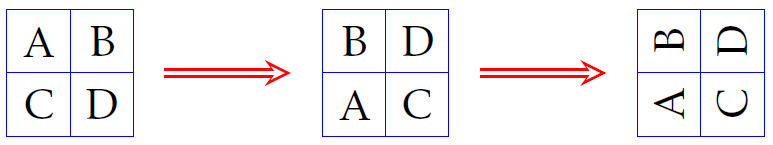
\includegraphics[width=.95\linewidth]{images/fig_02}
%\end{center}
%
%On supposera dans tout l’exercice que n est une puissance de 2.
%
%\subparagraph{}\textit{Exprimer en fonction de n le nombre de fois que la fonction blit est utilisée.}
%
%\subparagraph{}\textit{Quel est le coût total de cet algorithme lorsque le coût d’un blit d’un bloc 
%$k \times k$ est en $\mathcal{O}(n^2)$ ?}
%
%\subparagraph{}\textit{Et lorsque ce coût est en $\mathcal{O}(n)$  ?}
%
%\subparagraph{}\textit{En supposant qu’une image est représentée par une matrice numpy 
%$n \times n$, rédiger une fonction qui adopte cette
%démarche pour effectuer une rotation de 90\textdegree dans le sens direct (on simulera un blit par la copie d’une partie de la matrice vers une autre en décrivant ces parties par le slicing).}

%
%\section*{Exercice 5}
%\setcounter{subparagraph}{0}
%
%On suppose disposer d’une fonction \textsl{circle([x, y], r)} qui trace à l’écran un cercle de centre
%$(x;y)$ de rayon $r$. 
%\subparagraph*{}
%\textit{Définir deux fonctions récursives permettant de tracer les dessins présentés figure suivante (chaque cercle est de rayon moitié moindre qu’à la génération précédente).}
%
%\begin{center}
%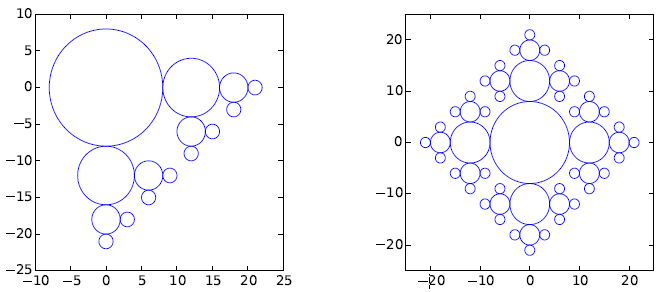
\includegraphics[width=.95\linewidth]{images/fig_03}
%% Le résultat des fonctions bubble1(4) et de bubble2(4).
%\end{center}


\section*{Exercice 4}
\setcounter{subparagraph}{0}

%\subparagraph{}\textit{}
On suppose disposer d’une fonction \textsf{polygon([xa, ya], [xb, yb], [xc, yc])} qui trace le
triangle plein dont les sommets ont pour coordonnées $(x_a;y_a)$, $(x_b;y_b)$, $(x_c;y_c)$. 
\subparagraph{}
\textit{Définir une fonction récursive permettant le tracé présenté figure suivante (tous les triangles sont équilatéraux).}

\begin{center}
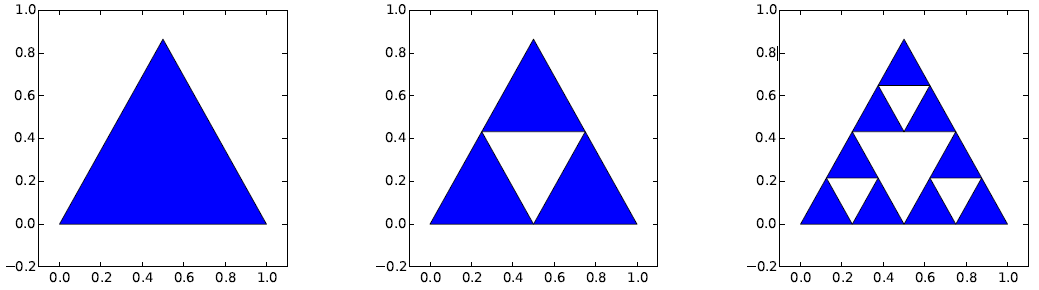
\includegraphics[width=.95\linewidth]{images/fig_04}
%Le résultat des fonctions sierpinski(n) pour n = 1;2; 3.
\end{center}

\ifprof
\begin{corrige}
\begin{python}
import numpy as np
import matplotlib.pyplot as plt

def triangle(A,B,C):
    """
    Entrées :
     * A,B,C : couples de coordonnées des points A B et C
    Sortie : 
     * Rien (plot) 
    """
    X,Y = [],[]
    X.append(A[0])
    X.append(B[0])
    X.append(C[0])
    Y.append(A[1])
    Y.append(B[1])
    Y.append(C[1])
    plt.fill(X,Y,'b')

#triangle((0,0),(1,0),(.5,np.sqrt(3)/2))

def trace(n,A,B,C):
    if n==1:
        triangle(A,B,C)
    else :
        a = (.5*(B[0]+C[0]),.5*(B[1]+C[1]))
        b = (.5*(C[0]+A[0]),.5*(C[1]+A[1]))
        c = (.5*(A[0]+B[0]),.5*(A[1]+B[1]))
        trace(n-1,A,c,b)
        trace(n-1,c,B,a)
        trace(n-1,b,a,C)
        
trace(4,(0,0),(1,0),(.5,np.sqrt(3)/2))        
\end{python}
\end{corrige}
\else
\fi
%\section*{Exercice 1 -- Suite de Fibonacci}
%\section*{Exercice 2 -- Recherche dichotomique}
%\section*{Exercice 3 -- Courbe du Dragon}




